% Cover letter: R&D Product Designer (R&D/Innovation Management, RPSI, remote), Amcor
% CV: Sections/cv_rd_product_designer.tex -> cv_gen/cv_giovanni_tauro-amcor.pdf
\documentclass[11pt,a4paper,sans]{moderncv}
% Shared preamble and header for the cover letters.
% One main file per application: cl_<company>.tex, built to
% cv_gen/coverletter_giovanni_tauro-<company>.pdf next to cv_giovanni_tauro-<company>.pdf.
% Paths (cl_gen/..., Pictures/...) are relative to the project root, as in the CV (see .latexmkrc).

\moderncvstyle{classic}
\moderncvcolor{blue}

\usepackage[scale=0.80]{geometry}
\setlength{\footskip}{136.00005pt}

\usepackage{fontawesome5}
% hyperref is loaded by moderncv itself; loading it here causes an option clash
\usepackage{xcolor}
\usepackage{graphicx}
\ifxetexorluatex
  \usepackage{fontspec}
  \usepackage{unicode-math}
  \defaultfontfeatures{Ligatures=TeX}
  \setmainfont{Latin Modern Roman}
  \setsansfont{Latin Modern Sans}
  \setmonofont{Latin Modern Mono}
  \setmathfont{Latin Modern Math}
\else
  \usepackage[T1]{fontenc}
  \usepackage{lmodern}
\fi

\usepackage[english]{babel}

% used for the PDF title and the letter closing; the visible header is \clheader below
\name{Giovanni}{Tauro}

% Header: #1 = headline under the name (same as the headline of the matching CV)
\newcommand{\clheader}[1]{%
\noindent
\begin{minipage}[c]{0.74\textwidth}
    {\Huge \textbf{Giovanni Tauro}}\\[-0.2em]
    {\small #1}\\[0.3em]

    \footnotesize
    \faMapMarker*~
    \href{https://www.google.com/maps/search/?api=1&query=Lecco+23900+Italy}
    {\color{blue}Bari-Lecco, Italy}
    \quad
    \faPhone*~
    \href{https://wa.me/393279437161}
    {\color{blue}+39 3279437161}
    \quad
    \faEnvelope~
    \href{mailto:giovanni.taurodi@gmail.com}
    {\color{blue}giovanni.taurodi@gmail.com}
    \\[-0.1em]

    \faLinkedin~
    \href{https://www.linkedin.com/in/giovanni-tauro-gt/}
    {\color{blue}LinkedIn}
    \quad
    \faGithub~
    \href{https://github.com/jotades}
    {\color{blue}GitHub}
    \quad
    \faGraduationCap~
    \href{https://scholar.google.com/citations?user=BS0aVGgAAAAJ&hl=it}
    {\color{blue}Scholar}
    \quad
    \faFilePdf~
    \href{https://www.notion.so/Giovanni-Tauro-2a7901d92f3a800b892af425c5875c6a}
    {\color{blue}Portfolio}
    \quad
    \faCubes~
    \href{https://grabcad.com/giovanni.tauro-3}
    {\color{blue}GrabCAD}

\end{minipage}
\hfill
\begin{minipage}[c]{0.18\textwidth}
    \raggedleft
    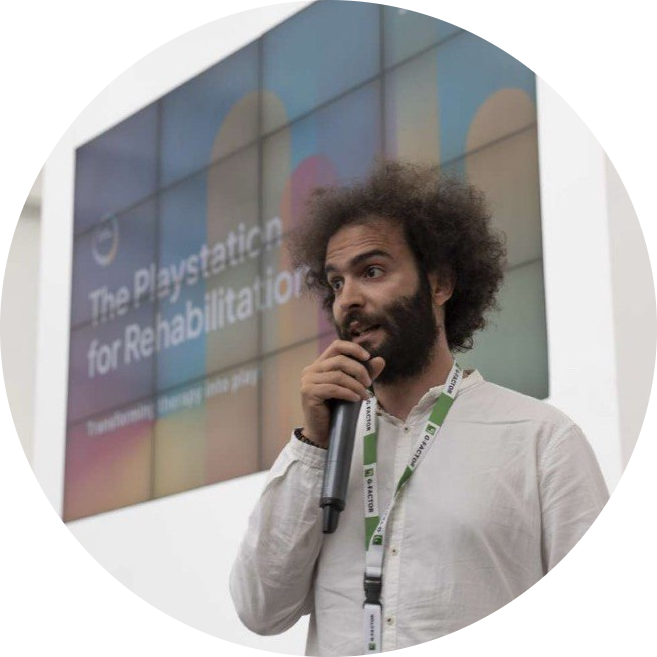
\includegraphics[width=2.8cm]{Pictures/Giovanni_pitch}
\end{minipage}
\vspace{0.1em}
}

\makeatletter
% the sender details are already in \clheader, so skip moderncv's own block
\@detailsfalse
% closing phrase, signature, name
\renewcommand*{\makeletterclosing}{%
  \@closing\\[0.6em]%
  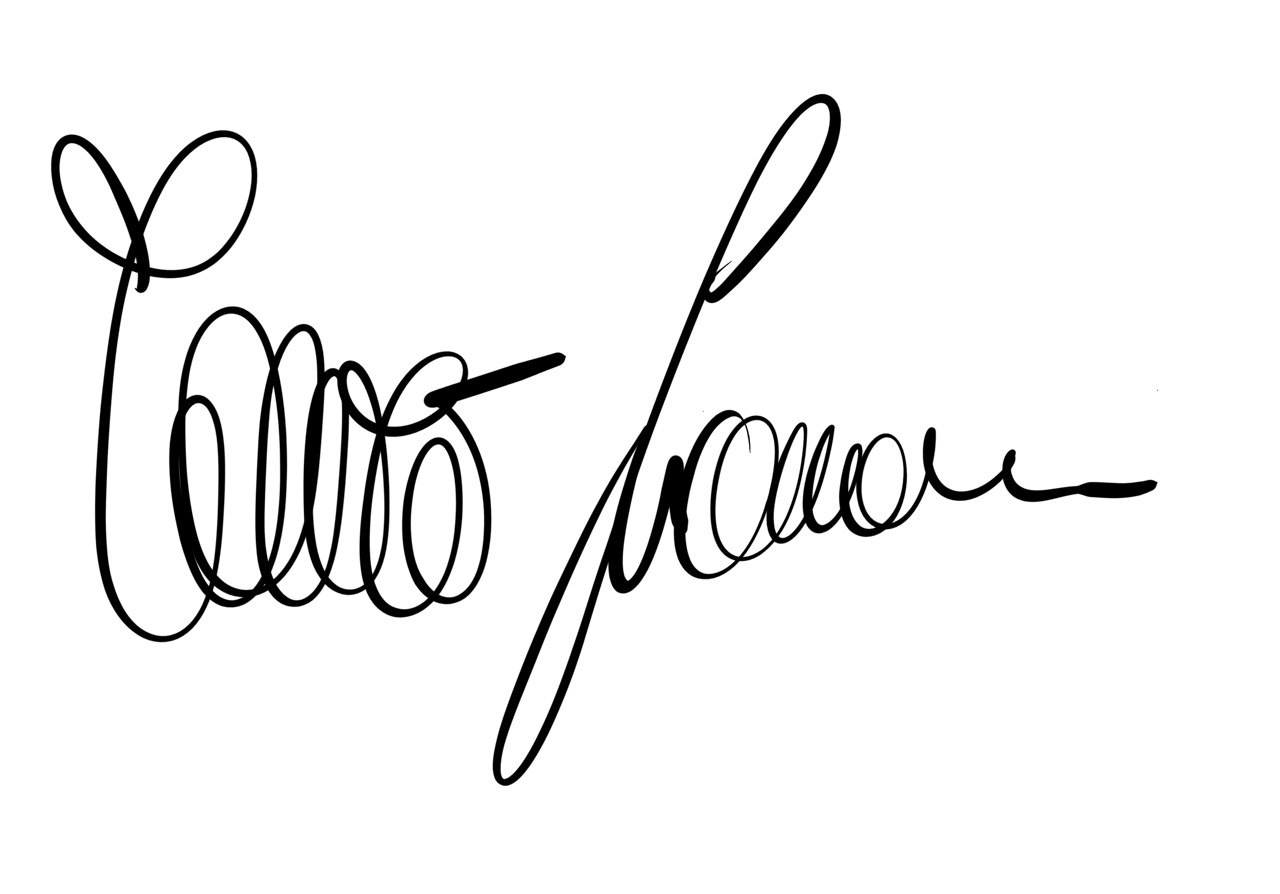
\includegraphics[height=1.2cm]{Pictures/sign_gt.jpg}\\[0.2em]%
  {\bfseries\@firstname~\@lastname}}
\makeatother


\begin{document}

\clheader{R\&D Product Designer | CAD, Prototyping \& Testing}

\recipient{R\&D / Innovation Management}{Amcor}
\opening{Dear Hiring Team,}
\closing{Sincerely,}
\makelettertitle

I am applying for the R\&D Product Designer role in the RPSI division. I trained as an industrial designer (BSc, University of Florence; MSc in Design \& Engineering, Politecnico di Milano) and for more than five years I have taken physical products from concept to tested prototype at CNR-STIIMA, the Italian National Research Council, and as Head of Product and co-founder of Rehabilia Technologies.

My main project is PhiCube, a modular rehabilitation device. I worked on it from user research and concept sketches to mechanical design, assembly and deployment in Italian clinics, and I am a co-inventor on its patent (WO2023214349A1). It reached a usability score of 85.8/100 (SUS) with 19 children and is now in two ongoing multicentre studies with 134 patients. For the Giocabile project I designed parametric, 3D-printed accessories for the same device, aimed at children with cerebral palsy.

The cycle your KPIs describe, from idea to prototype to a test that decides the next stage, is the one I work in every day. I model in SolidWorks and Fusion 360, build and assemble prototypes with 3D printing, choose materials and manufacturing methods by batch size, cost and technical constraints, then test with users and iterate on the results. I also write the documentation that goes with it, including CE-oriented technical files and manuals. Speed matters too: at an LMU Munich hardware challenge my team went from idea to a working rehabilitation prototype in 24 hours.

As Head of Product I set requirements, priorities and milestones with engineering, design and clinical partners, coordinate external suppliers, and keep several workstreams moving at once. Before that I worked as a product designer for Adidas, developing concepts from trend and competitor research and defining materials and colours, and as a freelancer turning 3D scans into production-ready CAD models.

My products so far are medical and rehabilitation devices rather than packaging, and I render in Blender rather than KeyShot. The fundamentals carry over: user needs, materials, manufacturability, testing and cost, in regulated settings where safety comes first. I am based in Italy and used to working remotely with partners in other countries.

I would welcome the chance to discuss the role further.

\makeletterclosing

\end{document}
